Рассмотрим более практичный подход, учитывающий все рассмотренные ранее аспекты.
Применяя современные фреймворки, такие как ASP.NET Core и Angular, можно реализовать следующий флоу аутентификации
в соответствии с приведенной ниже схемой
\begin{figure}[H]
    \centering
    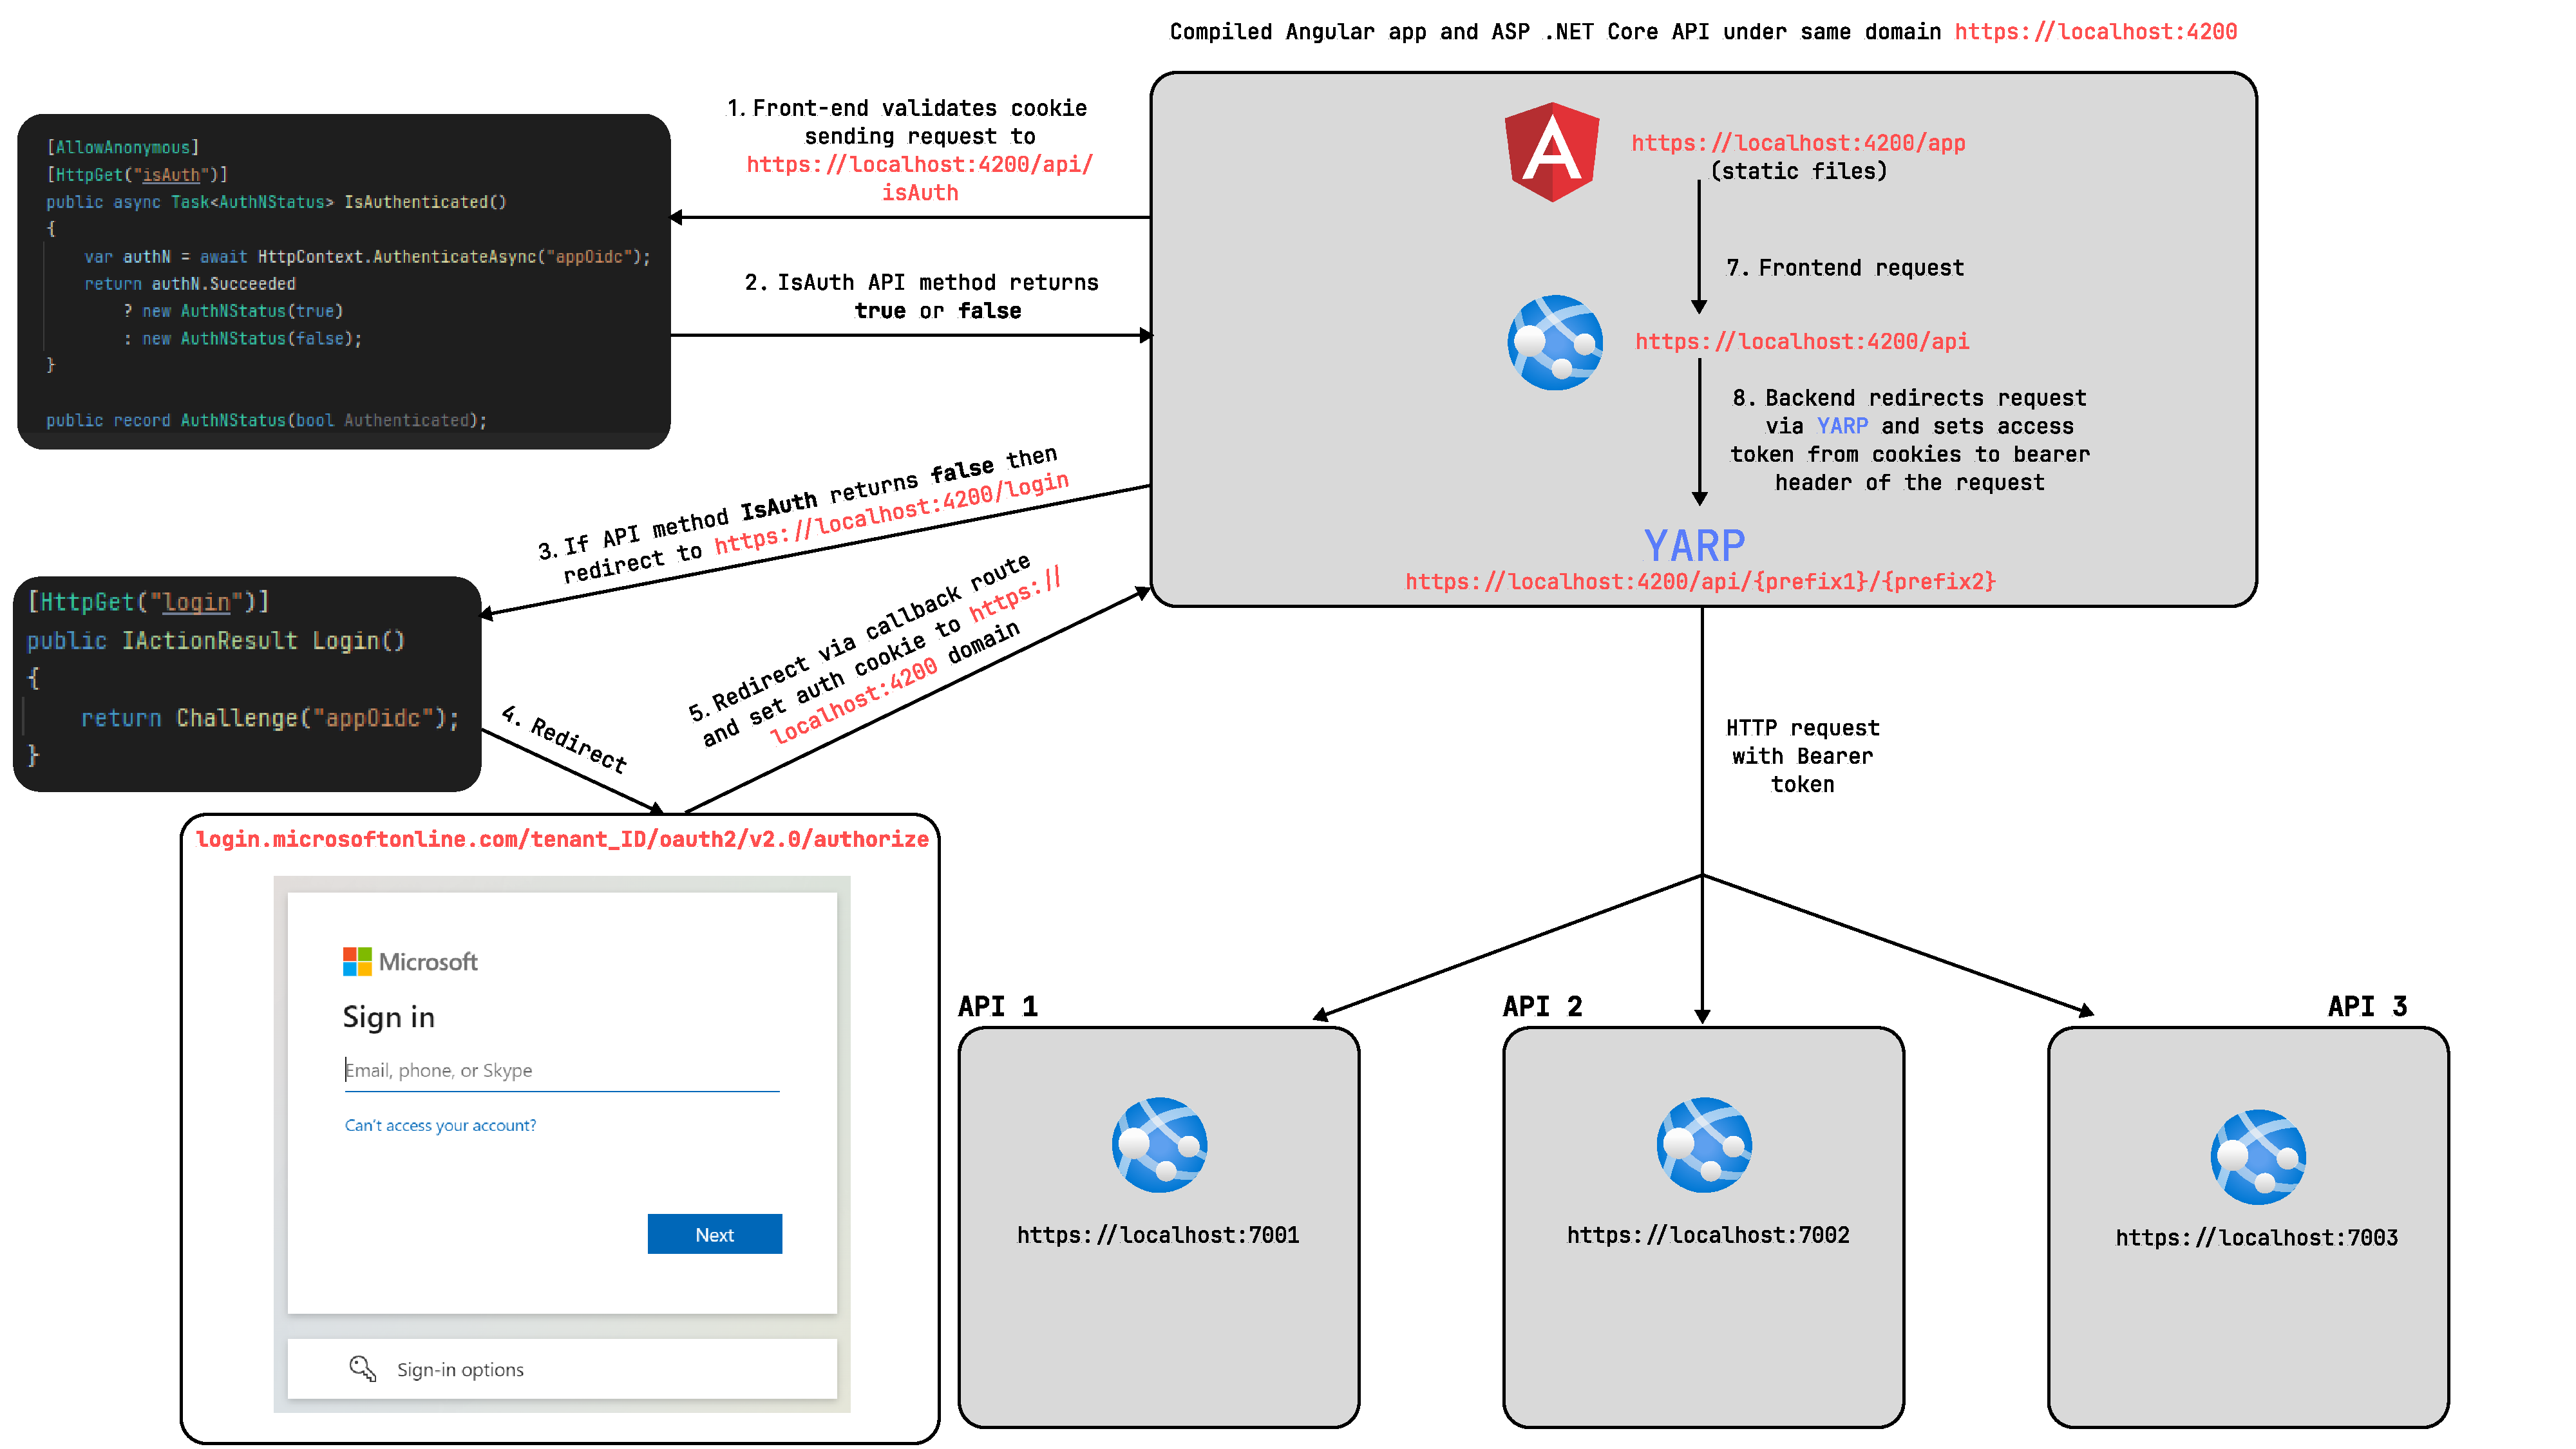
\includegraphics[width=1\textwidth]{img/Auth_flow_updated}
    ~\caption{Authentication flow diagram.}\label{fig:figure}
\end{figure}

Таким образом, весь процесс аутентификации можно описать в виде восьми этапов, таких как
\begin{enumerate}
    \item Скомпилированное Angular-приложение отправляет запрос к ендпоинту ASP.NET Core API для проверки текущего
    состояния аутентификации.
    Angular-приложение представляет собой набор предварительно скомпилированных пакетов, которые раздаются через
    тот же ASP.NET Core API на ендпоинте \texttt{/app}, что позволяет отказаться от кросс-доменных запросов и
    надежно хранить токены в файлах cookie.
    \item Ендпоинт ASP.NET Core API отвечает либо со HTTP статус кодом \texttt{200 (OK)} или \texttt{401 (Unauthorized)}
    \item Если на предыдущем шаге получен статусный код \texttt{401 (Unauthorized)}, то браузер перенаправляется
    на ендпоинт \texttt{/login} API ASP.NET Core, в ином случае пользователь получает доступ к защищенным ресурсам
    \item Метод Login ASP.NET Core приложения перенаправляет браузер на сайт авторизации
    Azure AD \texttt{login.microsoftonline.com/tenant/oauth2/v2.0/authorize}, где пользователь вводит свои учетные данные.
    Важно уточнить, что для получения ID-токена нам необходимо поместить параметр \texttt{openid} в область видимости (scope)
    \begin{spverbatim}
    serviceCollection
    .AddAuthentication(options => {...})
    .AddCookie(CookieAuthenticationDefaults.AuthScheme,
        options => {...})
    .AddOpenIdConnect(AuthConstants.AppOidc, options =>
    {
        ...
        options.Scope.Add("openid");
    });
\end{spverbatim}
    \item После успешной аутентификации на стороне Azure AD, браузер перенаправляется уже с установленными
    файлами cookie на \texttt{callback\_url}, который определен при регистрации приложения в Azure AD\@.
    В этот момент в флоу включается \texttt{TickerStore}~\cite{microsoftIticketstore2023, ticketStore_2023},
    который нужен для управления сессиями пользователей.
    Каждая сессия хранится в базе данных как сущность \texttt{UserSessionEntity}.
    \begin{spverbatim}
    public class UserSessionEntity
    {
        public Guid Id { get; set; }
        public DateTimeOffset CreatedAt { get; set; }
        public DateTimeOffset ExpiresAt { get; set; }
        public DateTimeOffset UpdatedAt { get; set; }
        public DateTimeOffset DateOfLastAccess { get; set; }
        public byte[] Value { get; set; }
    }
\end{spverbatim}
    Свойство Value типа \texttt{byte[]} содержит сериализованный \texttt{AuthenticationTicket}~\cite{microsoftAuthenticationTicket2023}
    объект, содержащий всю необходимую информацию, такую как ID-токен,
    токен доступа (access token) и токен обновления (refresh token).
    Класс \texttt{TickerStore} реализует интерфейс \texttt{ITickerStore}, который предлагает 4 метода:
    \texttt{StoreAsync, RenewAsync, RetrieveAsync, RemoveAsync}.
    \begin{itemize}
        \item Метод \texttt{StoreAsync} выполняется сразу после аутентификации на сервере авторизации, он сохраняет
        сессию пользователя в базе данных.
        \item Метод \texttt{RenewAsync} в нашем случае используется фоновым сервисом для обновления пользовательских сессий.
        \item Метод \texttt{RetrieveAsync} выполняется каждый раз, когда запрос отправляется на ендпоинт,
        помеченный \texttt{[Authorize]} атрибутом.
        \item Метод \texttt{RemoveAsync} выполняется по истечении срока действия cookie-файлов, а также используется
        тем же \texttt{RefreshBackgroundService} для удаления сессий, которые не использовались в течение длительного времени.
    \end{itemize}
    Пример реализации \texttt{TicketStore} можно найти на~\cite{ticketStore_2023}.
    Пример инъекции зависимостей (DI) \texttt{TicketStore} можно найти на~\cite{ticketStoreDI_2023}.
    На этом шаге происходит настройка аутентификационных cookie.
    \item Шаг 1 здесь повторяется, но теперь HTTP-запрос обязательно должен быть с кодом состояния \texttt{200 (OK)}.
    \item Скомпилированное фронтенд-приложение Angular отправляет запрос к ASP.NET Core API c cookie-файлами.
    Микросервис, принимающий запрос, используя библиотеку \texttt{YARP}~\cite{microsoftYarp2021}, вынимает из
    cookie файлов токен доступа и кладет его в заголовок, после чего перенаправляет запрос на один из микросервисов.
    Конфигурация \texttt{YARP} осуществляется в соответствии с~\cite{yarpDI_2023,yarpSectionAppSettings_2023}.
    \item Если на предыдущем шаге был получен статусный код \texttt{401 (Unauthorized)}, то шаг 1 повторяется.
\end{enumerate}